\section{BERTopic}

\textit{BERTopic} --- это метод моделирования тем, который использует трансформеры и \textit{c-TF-IDF} для создания плотных кластеров, позволяющих легко интерпретировать темы, сохраняя при этом важные слова в описаниях тем \cite{bib234234}. 

\subsection{Алгоритм}

\begin{figure}[H]
\centering
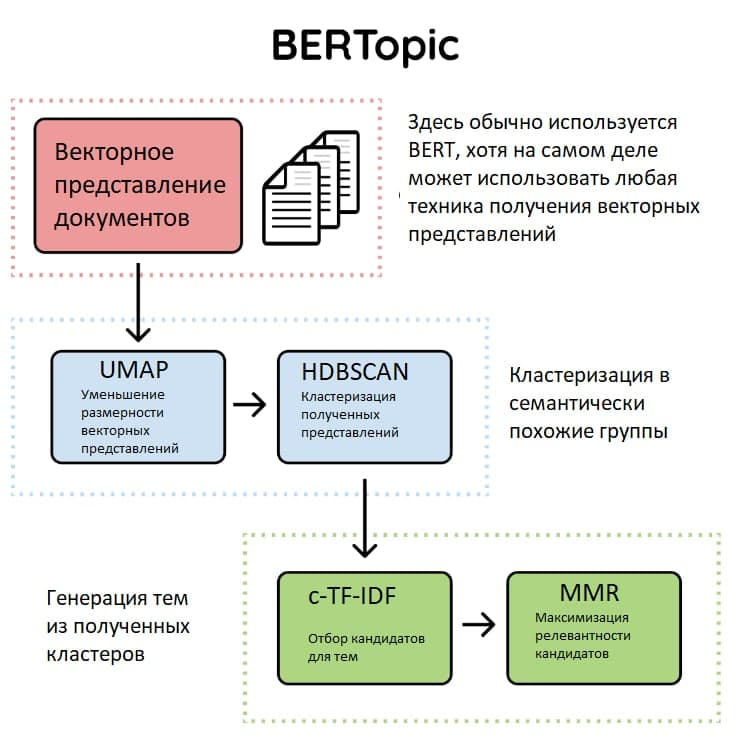
\includegraphics[scale=0.7]{pics/bertopic.jpg}
\caption{Стадии работы алгоритма \textit{BERTopic}}
\end{figure}

Алгоритм состоит из 3 шагов:

\begin{enumerate}

\item Первый шаг, который требуется сделать -- это преобразовать документы в числовые данные. Для этой цели используется \textit{BERT}, который извлекает различные векторные представления слов в зависимости от контекста. Это одна из лучших моделей в настоящее время для многих задач, связанных с текстом. \textit{BERT} получил награду за лучшую работу на ежегодной конференции североамериканского отделения  компьютерной лингвистики 2019 года \cite{bib_1} \cite{bib_2}.

\item Далее необходимо убедиться, что документы с похожим смыслом сгруппированы вместе, чтобы мы могли найти темы в этих кластерах. Перед этим нам сначала нужно снизить размерность векторных представлений слов, поскольку многие алгоритмы кластеризации плохо справляются с высокой размерностью. 
\textit{UMAP} --- это один из немногих алгоритмов уменьшения размерности, он является наиболее эффективным,
 поскольку он сохраняет значительную часть многомерной локальной структуры в более низкой размерности. 


После уменьшения размерности встраиваемых документов  мы можем кластеризовать документы с помощью \textit{HDBSCAN} (\textit{Hierarchical Density-Based Spatial Clustering of Applications with Noise}).
\textit{HDBSCAN} основан на алгоритме \textit{DBSCAN} и, как и другие алгоритмы кластеризации, используется для группировки данных \cite{bib_3}.

Помимо того, что он обычно показывает лучшее качество, он также быстрее, чем обычный 
\textit{DBSCAN}. Ниже приведен график нескольких алгоритмов кластеризации. При отметке в 200 000 объектов \textit{DBSCAN} занимает примерно вдвое больше времени, чем 
\textit{HDBSCAN}. Стоит отметить, что по мере увеличения количества объектов разница в производительности будет и дальше увеличиться в пользу \textit{HDBSCAN}:
\newline

\begin{figure}[H]
\centering
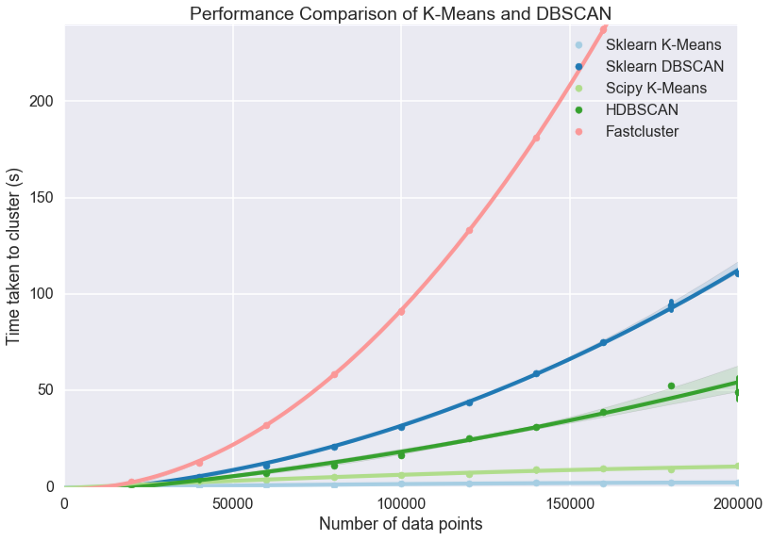
\includegraphics[scale=0.5]{pics/clustering-comparison.png}
\caption{Сравнение производительности алгоритмов кластеризации}
\end{figure}

\textit{HDBSCAN} --- алгоритм кластеризации, который довольно хорошо работает с 
\textit{UMAP}, поскольку \textit{UMAP} поддерживает большую локальную структуру даже в пространстве меньшей размерности. Более того, \textit{HDBSCAN} не переносит отдельные точки в кластеры, поскольку считает их выбросами.

\item Теперь мы сгруппировали похожие документы вместе, которые должны представлять темы, из которых они состоят. Что мы хотим узнать из созданных нами кластеров --- это то, что отличает один кластер по своему содержанию от другого.  Как мы можем извлечь темы из сгруппированных документов? Чтобы решить эту проблему, используется классовый вариант 
\textit{TF-IDF} (\textit{c-TF-IDF}), который позволил бы извлечь то, что делает каждый набор документов уникальным по сравнению с другим. Интуиция, лежащая в основе метода, заключается в следующем: когда мы применяем \textit{TF-IDF} как обычно к набору документов, мы в сравниваем важность слов среди всех документов, а в классовом варианте теперь у нас есть одно значение важности для каждого слова в кластере, которое можно использовать для создания темы. Если мы возьмем несколько  самых важных слов в каждом кластере, то получим хорошее представление о кластере и, следовательно, теме.

Чтобы создать эту оценку классового \textit{TF-IDF}, сначала нужно создать один документ для каждого кластера документов.
%\begin{verbatim}
%docs_df = pd.DataFrame(data, columns=["Doc"])
%docs_df['Topic'] = cluster.labels_
%docs_df['Doc_ID'] = range(len(docs_df))
%docs_per_topic = docs_df.groupby(['Topic'], as_index = False) \
%.agg({'Doc': ' '.join})
%\end{verbatim}
Затем мы применяем \textit{TF-IDF} на основе классов:

\begin{center}
$\textit{c-TF-IDF}_{i} = 
\dfrac{t_i}{w_i} \cdot 
\log{
\dfrac{m}{\sum\limits_j^n t_j}}$
\end{center}

Где частота каждого слова $t$ извлекается для каждого класса $i$ и делится на общее количество слов $w$ в классе. Это действие можно рассматривать как форму регуляризации частых слов в классе. Затем общее количество документов $m$ делится на общую частоту слова $t$ по всем $n$ классам.

Теперь у нас есть одно значение важности для каждого слова в кластере, которое можно использовать для создания темы. После обучения нашей модели мы можем итеративно пройти, возможно, сотню тем, чтобы получить хорошее представление о темах, которые были извлечены. Однако это занимает некоторое время и не имеет глобального представления. Вместо этого мы можем визуализировать темы. 

\end{enumerate}

\subsection{Интерпретация работы алгоритма} 

Для визуализации работы алгоритмы используется представление тем в 
\textit{2D} с помощью \textit{UMAP}, который создает двумерную проекцию всех точек и затем визуализирует эти два измерения, причем в интерактивном виде, что позволяет нам получить представление, понятное человеку. Пример визуализации от авторов алгоритма \cite{bib_4}:


\begin{figure}[H]
\centering
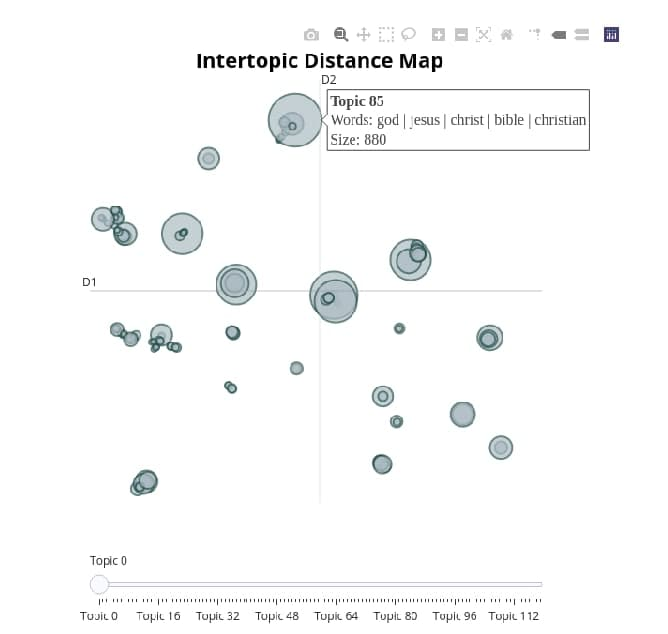
\includegraphics[scale=0.9]{pics/bertopic-visual-1.jpg}
\caption{Пример визуализации тем в $BERTopic$}
\end{figure}

На картинке видно, что кластеры довольно равномерно распределились по пространству и кластера действительно очень интерпремируемы: например, на рисунке показан кластер религиозных слов.

Мы также можем рассчитать вероятность того, что темы могут быть найдены в документе. Эти вероятности означают, насколько \textit{BERTopic} 
уверен в том, что определенные темы могут быть найдены в документе \cite{bib_4}:


\begin{figure}[H]
\centering
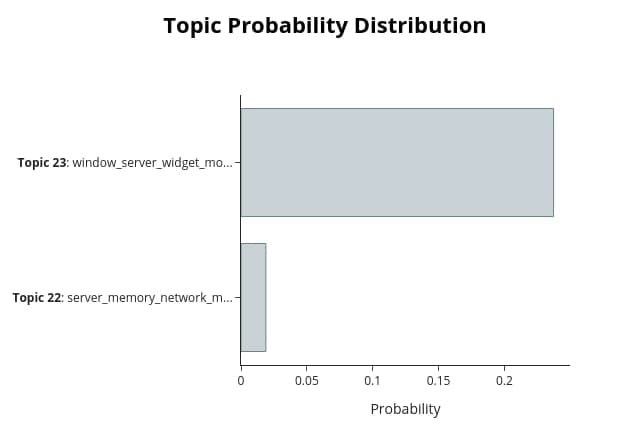
\includegraphics[scale=0.9]{pics/bertopic-visual-2.jpg}
\caption{Пример распределения вероятностей тем в $BERTopic$}
\end{figure}


Важно понимать, что распределение вероятностей не указывает на распределение частотности тем в документе. Это просто показывает, насколько 
\textit{BERTopic} уверен в том, что в документе можно найти определенные темы.
